\section{Programmation asynchrone}
\label{sec:async}

L'un des objectifs principales du logiciel est de garantir une fréquence de mesure
des capteurs la plus élevée possible. Pour cela, le programme doit être capable
d'effectuer plusieurs tâches en parallèle. En effet par exemple, l'envoi d'un message
de télémesure par LoRa prend un certain temps durant lequel le programme ne doit pas
être bloqué. Pour cela, les différentes tâches seront exécutées de manière asynchorne
\footnote{La programmation asynchrone est un modèle de programmation qui donne l'illusion
qu'un ordinateur effectue plusieurs tâches en parallèle, sans attendre la fin de chaque
tâche avant de passer à la suivante.} et non nécessairement séquentiellement.\\

Dans le cas de l'OMEGAAA, l'architecture asynchrone se caractérise par deux objets :
\begin{itemize}
    \item Les tâches : ce sont les différentes actions que le programme peut effectuer
    en parallèle.
    \item L'ordonanceur : c'est une structure contenant notamment les tâches à exécuter.
\end{itemize}

\subsection{Une tâche (TASK)}
\label{subsec:task}

Contrairement à une fonction classique, une tâche est une fonction qui peut commencer,
interrompre et reprendre son exécution en plusieurs temps. Dans l'OMEGAAA, une tâche se
matérialise par une structure de données contenant trois éléments : une fonction classique
(\texttt{func}\footnote{\label{footnote:ref_async_h}cf Code \ref{lst:async_h}}), un indice
de référence(\texttt{idx}\footnoteref{footnote:ref_async_h}) et une sous-structure de données
appelée "contexte d'exécution" (\texttt{context}\footnoteref{footnote:ref_async_h}).
Le contexte d'exécution contient les informations nécessaires pour reprendre l'exécution de
la tâche là où elle s'était arrêtée auparavant.

Par simplicité et pour des raisons de performances, bien que chaque type de tâche a besoin
d'un contexte d'exécution unique, \texttt{context} est une zone mémoire de taille fixe.
Cette taille est définie par la constante \texttt{ASYNC\_CONTEXT\_DEFAULT\_BYTES\_SIZE}
\footnoteref{footnote:ref_async_h} et est par défaut de 64 octets. Cela permet d'uniformiser
la structure de toutes les tâches. Cette taille doit être suffisante pour contenir le contexte
d'exécution de n'importe quelle tâche et doit être redéfini en fonction des besoin du programme
tout en considérant les limites de mémoire du microcontrôleur.
\subsection{L'ordonanceur (SCHEDULER)}
\label{subsec:scheduler}
L'ordonanceur est une structure de données qui contient les tâches à exécuter. Il se
matérialise par une structure contenant quatre éléments : le nombre de tâches en cours
d'exécution (\texttt{length}\footnoteref{footnote:ref_async_h}), l'indice de la tâche
actuellement en cours d'exécution (\texttt{current\_idx}\footnoteref{footnote:ref_async_h}),
le nombre de tâches exécutées depuis le dernier tour de boucle (\texttt{nbr\_has\_run\_task}
\footnoteref{footnote:ref_async_h}), un tableau de pointeurs de tâches (\texttt{tasks}
\footnoteref{footnote:ref_async_h}) et un tableau de booléens indiquant quels sont les pointeurs
du tableau \texttt{tasks} faisant référence à des tâches en cours d'exécution (\texttt{running}
\footnoteref{footnote:ref_async_h}). L'ordonanceur gère également la zone mémoire allouée dans
le tas pour les tâches. Il ne peut gérer qu'un nombre limité de tâches définie par la constante
\texttt{MAX\_TASKS\_NBR}\footnoteref{footnote:ref_async_h} et vaut par défaut 50. Là aussi, si
plus (ou moins) de tâches seront exéctutées en parallèle, il est nécessaire de redéfinir cette
constante en conséquence.

\begin{figure}[h]
    \centering
    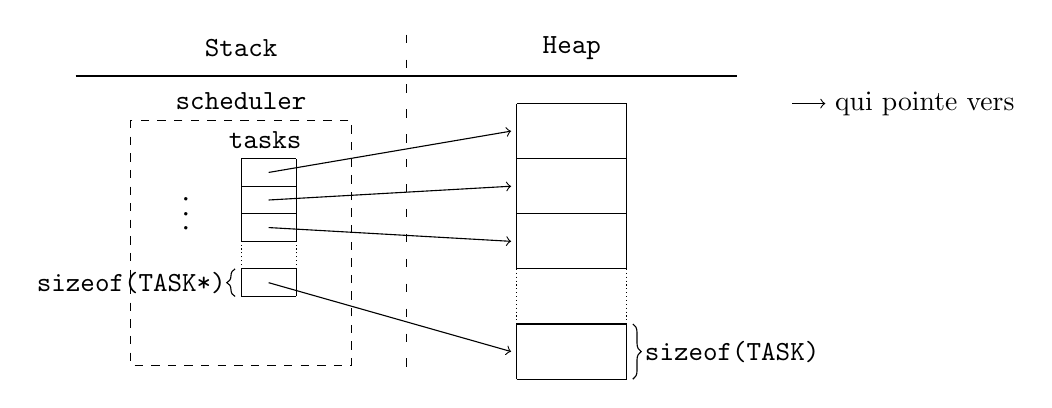
\begin{tikzpicture}[yscale=0.70, xscale=1.4]
        % \draw[help lines] (-6,-3) grid (0, 3);

        \draw node at (-4.5, 3) {\texttt{Stack}};
        \draw node at (-1.5, 3) {\texttt{Heap}};

        \draw (-6, 2.5) -- (0, 2.5);
        \draw[loosely dashed] (-3, 3.25) -- (-3, -3);

        \draw node at (-4.5, 2.05) {\texttt{scheduler}};

        \draw node[anchor=south west] at (-4.7, 1) {\texttt{tasks}};
        \draw[step=0.5] (-4.5, -0.5) grid (-4.0,  1);
        \draw[step=0.5] (-4.5, -1.5) grid (-4.0, -1);
        \draw[densely dotted] (-4.5, -1) -- (-4.5, -0.5);
        \draw[densely dotted] (-4.0, -1) -- (-4.0, -0.5);

        \draw node[rotate=90] at (-5.0, 0) {\texttt{...}};

        % \draw[dashed] (-5.5, 2.25) -- (-3.5, 2.25) -- (-3.5, -2.75) -- (-5.5, -2.75) -- cycle;
        \draw[dashed] (-5.5, 1.7) rectangle (-3.5, -2.75);

        \draw (-2, +2) grid (-1, -1);
        \draw (-2, -2) grid (-1, -3);
        \draw[densely dotted] (-2, -1) -- (-2, -2);
        \draw[densely dotted] (-1, -1) -- (-1, -2);

        \draw[->] (-4.25, +0.75) -- (-2.05, +1.5);
        \draw[->] (-4.25, +0.25) -- (-2.05, +0.5);
        \draw[->] (-4.25, -0.25) -- (-2.05, -0.5);
        \draw[->] (-4.25, -1.25) -- (-2.05, -2.5);

        \draw [decorate,decoration={brace,amplitude=3pt,mirror,raise=0.5ex}]
        (-4.5, -1) -- (-4.5, -1.5) node[midway, anchor=east, xshift=-2]{\texttt{sizeof(TASK*)}};

        \draw [decorate,decoration={brace,amplitude=3pt,raise=0.5ex}]
        (-1, -2) -- (-1, -3) node[midway, anchor=west, xshift=3]{\texttt{sizeof(TASK)}};

        \draw[->] (0.5, 2) -- (0.8, 2) node[right] {qui pointe vers};

    \end{tikzpicture}
    \caption{L'agencement des tâches dans le tas et leur lien avec l'ordonanceur}
\end{figure}
\subsection{Exemple 1 : Ordonancement des tâches}
\label{subsec:exemple_1}

Pour mieux comprendre le fonctionnement de l'ordonanceur et des tâches, un exemple de scénario
d'utilisation est donné ci-dessous.\\

- En premier lieu, les tâches A, B, C, D et E sont ajoutées dans une zone mémoire alloué au moment de
l'initilisation de l'ordonanceur et leur addresse mémoire respective sont placées dans le tableau
\texttt{task}. Puisqu'elles sont toutes en cours d'exécution, les booléens correspondants à leur index
dans le tableau \texttt{running} sont à \texttt{true}. (L'addresse mémoire de chaque tâche sera noté
"\&X" où X est le nom de la tâche.) 

\begin{figure}[h]
    \centering
    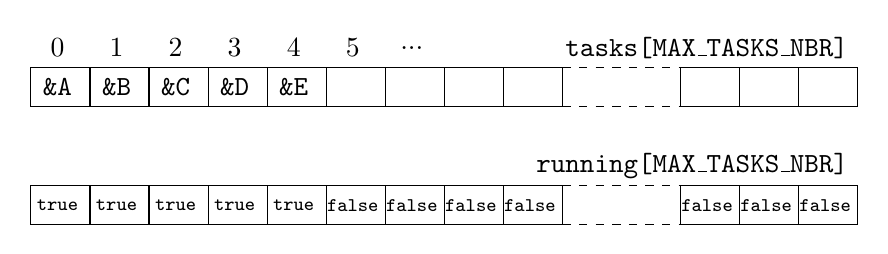
\begin{tikzpicture}[yscale=1, xscale=1.5]
        % \draw[help lines] (-5,-1) grid (5, 2);

        \draw node at (-4.775, 1.25) {0};
        \draw node at (-4.275, 1.25) {1};
        \draw node at (-3.775, 1.25) {2};
        \draw node at (-3.275, 1.25) {3};
        \draw node at (-2.775, 1.25) {4};
        \draw node at (-2.275, 1.25) {5};
        \draw node at (-1.775, 1.25) {...};

        \draw node[anchor=east] at (2, 1.25) {\texttt{tasks[MAX\_TASKS\_NBR]}};
        \draw[step=0.5] (-5.0, 0.5) grid (-0.5, 1);
        \draw[step=0.5] (+0.5, 0.5) grid (+2.0, 1);
        \draw[dashed] (-0.5, 1.0) -- (+0.5, 1.0);
        \draw[dashed] (-0.5, 0.5) -- (+0.5, 0.5);

        \draw node at (-4.775, 0.75) {\texttt{\&A}};
        \draw node at (-4.275, 0.75) {\texttt{\&B}};
        \draw node at (-3.775, 0.75) {\texttt{\&C}};
        \draw node at (-3.275, 0.75) {\texttt{\&D}};
        \draw node at (-2.775, 0.75) {\texttt{\&E}};
        
        \draw[step=0.5] (-5.0, -0.5) grid (-0.5, -1);
        \draw[step=0.5] (+0.5, -0.5) grid (+2.0, -1);
        \draw[dashed] (-0.5, -1.0) -- (+0.5, -1.0);
        \draw[dashed] (-0.5, -0.5) -- (+0.5, -0.5);
        \draw node[anchor=east] at (2, -0.25) {\texttt{running[MAX\_TASKS\_NBR]}};

        \draw node at (-4.775, -0.75) {\scriptsize\texttt{true}};
        \draw node at (-4.275, -0.75) {\scriptsize\texttt{true}};
        \draw node at (-3.775, -0.75) {\scriptsize\texttt{true}};
        \draw node at (-3.275, -0.75) {\scriptsize\texttt{true}};
        \draw node at (-2.775, -0.75) {\scriptsize\texttt{true}};
        \draw node at (-2.275, -0.75) {\scriptsize\texttt{false}};
        \draw node at (-1.775, -0.75) {\scriptsize\texttt{false}};
        \draw node at (-1.275, -0.75) {\scriptsize\texttt{false}};
        \draw node at (-0.775, -0.75) {\scriptsize\texttt{false}};
        \draw node at ( 0.725, -0.75) {\scriptsize\texttt{false}};
        \draw node at ( 1.225, -0.75) {\scriptsize\texttt{false}};
        \draw node at ( 1.725, -0.75) {\scriptsize\texttt{false}};
    \end{tikzpicture}
    \caption{Schéma des tableaux tasks et running de l'ordonanceur (1)}
    \label{fig:async_scheduler_0}
\end{figure}

- Ensuite, la tâche C se termine et se retire de l'ordonanceur. Son booléen correspondant dans
le tableau \texttt{running} est alors à \texttt{false}. Prenons cet exemple pour expliquer
comment les tâches sont exécutées par l'ordonanceur. A chaque fois que la fonction
\texttt{run\_scheduler}\footnoteref{footnote:ref_async_h} est appelée, l'ordonanceur exécute la tâche suivante. Cette dernière
correspond à la première tâche dont le booléen correspondant dans le tableau \texttt{running}
est à \texttt{true} depuis l'index \texttt{current\_idx} jusqu'à ce que l'ensemble des
tâches aient été exécutées. Dans le cas de la figure \ref{fig:async_scheduler_1}, au premier
tour de boucle, la tâche A est exécutée, puis la tâche B, puis la tâche D et enfin la tâche E.
La tâche C n'est pas exécutée car son booléen correspondant dans le tableau \texttt{running}
est à \texttt{false}. \texttt{current\_idx} passe alors respectivement de 0, 1, 3, et 4.
Ensuite, puisque toutes les tâches ont été parcourues une fois, la tâche suivante est la tâche
A. Cela est répété jusqu'à ce que toutes les tâches soient retirées de l'ordonanceur.

\begin{figure}[h]
    \centering
    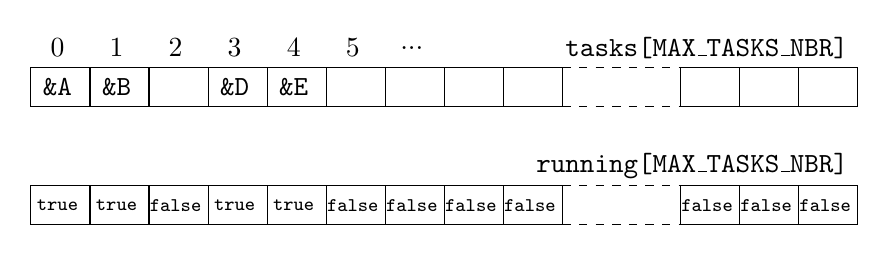
\begin{tikzpicture}[yscale=1, xscale=1.5]
        % \draw[help lines] (-5,-1) grid (5, 2);

        \draw node at (-4.775, 1.25) {0};
        \draw node at (-4.275, 1.25) {1};
        \draw node at (-3.775, 1.25) {2};
        \draw node at (-3.275, 1.25) {3};
        \draw node at (-2.775, 1.25) {4};
        \draw node at (-2.275, 1.25) {5};
        \draw node at (-1.775, 1.25) {...};

        \draw node[anchor=east] at (2, 1.25) {\texttt{tasks[MAX\_TASKS\_NBR]}};
        \draw[step=0.5] (-5.0, 0.5) grid (-0.5, 1);
        \draw[step=0.5] (+0.5, 0.5) grid (+2.0, 1);
        \draw[dashed] (-0.5, 1.0) -- (+0.5, 1.0);
        \draw[dashed] (-0.5, 0.5) -- (+0.5, 0.5);

        \draw node at (-4.775, 0.75) {\texttt{\&A}};
        \draw node at (-4.275, 0.75) {\texttt{\&B}};
        \draw node at (-3.275, 0.75) {\texttt{\&D}};
        \draw node at (-2.775, 0.75) {\texttt{\&E}};
        
        \draw[step=0.5] (-5.0, -0.5) grid (-0.5, -1);
        \draw[step=0.5] (+0.5, -0.5) grid (+2.0, -1);
        \draw[dashed] (-0.5, -1.0) -- (+0.5, -1.0);
        \draw[dashed] (-0.5, -0.5) -- (+0.5, -0.5);
        \draw node[anchor=east] at (2, -0.25) {\texttt{running[MAX\_TASKS\_NBR]}};

        \draw node at (-4.775, -0.75) {\scriptsize\texttt{true}};
        \draw node at (-4.275, -0.75) {\scriptsize\texttt{true}};
        \draw node at (-3.775, -0.75) {\scriptsize\texttt{false}};
        \draw node at (-3.275, -0.75) {\scriptsize\texttt{true}};
        \draw node at (-2.775, -0.75) {\scriptsize\texttt{true}};
        \draw node at (-2.275, -0.75) {\scriptsize\texttt{false}};
        \draw node at (-1.775, -0.75) {\scriptsize\texttt{false}};
        \draw node at (-1.275, -0.75) {\scriptsize\texttt{false}};
        \draw node at (-0.775, -0.75) {\scriptsize\texttt{false}};
        \draw node at ( 0.725, -0.75) {\scriptsize\texttt{false}};
        \draw node at ( 1.225, -0.75) {\scriptsize\texttt{false}};
        \draw node at ( 1.725, -0.75) {\scriptsize\texttt{false}};

    \end{tikzpicture}
    \caption{Schéma des tableaux tasks et running de l'ordonanceur (2)}
    \label{fig:async_scheduler_1}
\end{figure}

- Depuis l'exemple ci-haut, les tâches F et G sont ajoutées à l'ordonanceur. L'ordonanceur cherche
alors la première place libre dans le tableau \texttt{tasks} pour y ajouter la tâche, soit le
premier index où le booléen correspondant dans le tableau \texttt{running} est à \texttt{false}.
Dans ce cas, c'est l'index 3. La tâche F est alors ajoutée à cet index et le booléen correspondant
dans le tableau \texttt{running} est mis à \texttt{true}. La tâche G est ajoutée de la même manière
à l'index 5.

\begin{figure}[h]
    \centering
    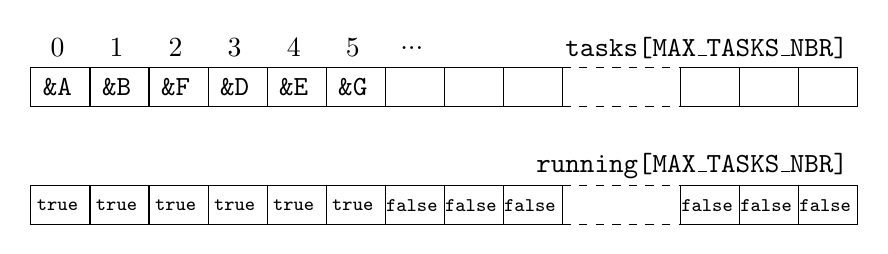
\begin{tikzpicture}[yscale=1, xscale=1.5]
        % \draw[help lines] (-5,-1) grid (5, 2);

        \draw node at (-4.775, 1.25) {0};
        \draw node at (-4.275, 1.25) {1};
        \draw node at (-3.775, 1.25) {2};
        \draw node at (-3.275, 1.25) {3};
        \draw node at (-2.775, 1.25) {4};
        \draw node at (-2.275, 1.25) {5};
        \draw node at (-1.775, 1.25) {...};

        \draw node[anchor=east] at (2, 1.25) {\texttt{tasks[MAX\_TASKS\_NBR]}};
        \draw[step=0.5] (-5.0, 0.5) grid (-0.5, 1);
        \draw[step=0.5] (+0.5, 0.5) grid (+2.0, 1);
        \draw[dashed] (-0.5, 1.0) -- (+0.5, 1.0);
        \draw[dashed] (-0.5, 0.5) -- (+0.5, 0.5);

        \draw node at (-4.775, 0.75) {\texttt{\&A}};
        \draw node at (-4.275, 0.75) {\texttt{\&B}};
        \draw node at (-3.775, 0.75) {\texttt{\&F}};
        \draw node at (-3.275, 0.75) {\texttt{\&D}};
        \draw node at (-2.775, 0.75) {\texttt{\&E}};
        \draw node at (-2.275, 0.75) {\texttt{\&G}};
        
        \draw[step=0.5] (-5.0, -0.5) grid (-0.5, -1);
        \draw[step=0.5] (+0.5, -0.5) grid (+2.0, -1);
        \draw[dashed] (-0.5, -1.0) -- (+0.5, -1.0);
        \draw[dashed] (-0.5, -0.5) -- (+0.5, -0.5);
        \draw node[anchor=east] at (2, -0.25) {\texttt{running[MAX\_TASKS\_NBR]}};

        \draw node at (-4.775, -0.75) {\scriptsize\texttt{true}};
        \draw node at (-4.275, -0.75) {\scriptsize\texttt{true}};
        \draw node at (-3.775, -0.75) {\scriptsize\texttt{true}};
        \draw node at (-3.275, -0.75) {\scriptsize\texttt{true}};
        \draw node at (-2.775, -0.75) {\scriptsize\texttt{true}};
        \draw node at (-2.275, -0.75) {\scriptsize\texttt{true}};
        \draw node at (-1.775, -0.75) {\scriptsize\texttt{false}};
        \draw node at (-1.275, -0.75) {\scriptsize\texttt{false}};
        \draw node at (-0.775, -0.75) {\scriptsize\texttt{false}};
        \draw node at ( 0.725, -0.75) {\scriptsize\texttt{false}};
        \draw node at ( 1.225, -0.75) {\scriptsize\texttt{false}};
        \draw node at ( 1.725, -0.75) {\scriptsize\texttt{false}};

    \end{tikzpicture}
    \caption{Schéma des tableaux tasks et running de l'ordonanceur (3)}
    \label{fig:async_scheduler_2}
\end{figure}
\subsection{Implémentation}
\label{subsec:implementation}

Ci-dessous est présenté le code source de la déclaration des fonctions principales associées à l'ordonanceur
et aux tâches. L'implémentation même de ces fonctions n'est pas présentée ici puisque jugé trop longue et
non essentielle à la compréhension du concept. L'implémentation complète est disponible dans le code source
du projet.

\begin{lstlisting}[style=prog, frame=shadowbox, caption={Définition des tâches et de l'ordonanceur (scheduler.h)}, label={lst:async_h},
    emph={[1]ASYNC_CONTEXT_DEFAULT_BYTES_SIZE, MAX_TASKS_NBR, init_scheduler, add_task, kill_task, run_task,
    run_scheduler}, emphstyle={[1]\color{C}},
    emph={[2]SCHEDULER, TASK, __task_func_t, task_func_t}, emphstyle={[2]\color{E}}]
#include <stdbool.h>
#include "stm32f4xx_hal.h"

#define ASYNC_CONTEXT_DEFAULT_BYTES_SIZE 64
#define MAX_TASKS_NBR 50

// fonction a executer (prend en param le scheduler et le contexte)
typedef void(*__task_func_t)(void*, void*);

typedef struct {
    __task_func_t   func;
    size_t          idx;
    bool           *is_done;
    uint8_t         context[ASYNC_CONTEXT_DEFAULT_BYTES_SIZE];
} TASK;

typedef struct {
    size_t   length;
    size_t   current_idx;
    size_t   nbr_has_run_task;
    TASK    *tasks[MAX_TASKS_NBR];
    bool     running[MAX_TASKS_NBR];
} SCHEDULER;

typedef void(*task_func_t)(SCHEDULER*, TASK*);


// Initialise l'ordonanceur notamment en allouant la zone mémoire pour les tâches.
void init_scheduler(SCHEDULER *scheduler);

// Initialise une tâche, la place dans la zone mémoire allouée, l'ajoute à la liste
// des tâches, met à jour le tableau running (active la tâche), les variables de
// l'ordonanceur et renvoie l'addresse mémoire de la tâche.
TASK *add_task(SCHEDULER *scheduler, task_func_t func);

// Met à jour le tableau running (désactive la tâche), les variables de l'ordonanceur
// et le drapeau "*is\_done" de la tâche s'il est défini.
void kill_task(SCHEDULER *scheduler, TASK *task);

// Exécute une tâche
void run_task(SCHEDULER *scheduler, TASK *task);

// Exécute la tâche suivante
void run_scheduler(SCHEDULER *scheduler);
\end{lstlisting}
\subsection{Exemple 2 : Création et logique d'une tâches}
\label{subsec:exemple_2}

Afin de mieux comprendre le fonctionnement de l'ordonanceur et des tâches, un exemple
d'implémentation est donné ci-dessous. Cet exemple est composé de deux tâches :
\begin{itemize}
    \item \texttt{task1} : une tâche qui créer la tâche 2 et affiche un message
    d'état du programme.
    \item \texttt{task2} : une tâche simulant une opération prenant du temps.
\end{itemize}
On suppose que la fonction \texttt{HAL\_GetTick} retourne le temps écoulé en millisecondes
depuis le démarrage du programme.

\begin{lstlisting}[style=prog, frame=shadowbox, caption={Exemple asynchrone}, label={lst:ex_async},
    emph={[1]ASYNC_task1, ASYNC_task2, ASYNC_task1_init, ASYNC_task2_init, init_scheduler, add_task, kill_task, run_task,
    run_scheduler, HAL_GetTick, printf}, emphstyle={[1]\color{C}},
    emph={[2]SCHEDULER, TASK, TASK1_STATE, ASYNC_task1_CONTEXT, ASYNC_task2_CONTEXT}, emphstyle={[2]\color{E}}]
#include <stdbool.h>
#include "stm32f4xx_hal.h"
#include "scheduler.h"

typedef enum {
    TASK1_INIT,
    TASK1_WAIT,
    TASK1_END
} TASK1_STATE;

typedef struct {
    TASK1_STATE state;
    bool        task2_done;
    uint32_t    last_time;
} ASYNC_task1_CONTEXT;

typedef struct {
    bool         started;
    uint32_t     delay;
    uint32_t     last_time;
} ASYNC_task2_CONTEXT;


void ASYNC_task1_init(TASK *task);
void ASYNC_task2_init(TASK *task, uint32_t delay);
void ASYNC_task1(SCHEDULER *scheduler, TASK *task);
void ASYNC_task2(SCHEDULER *scheduler, TASK *task);


// =========================================


void ASYNC_task1_init(TASK *task) {
    ASYNC_task1_CONTEXT *context = (ASYNC_task1_CONTEXT*)task->context;

    context->state = TASK1_STATE_INIT;
    context->task2_done = false;
    context->last_time = 0;
}

void ASYNC_task2_init(TASK *task, uint32_t delay) {
    ASYNC_task2_CONTEXT *context = (ASYNC_task2_CONTEXT*)task->context;

    context->started = false;
    context->delay = delay;
    context->last_time = 0;
}


void ASYNC_task1(SCHEDULER *scheduler, TASK *task) {
    ASYNC_task1_CONTEXT *context = (ASYNC_task1_CONTEXT*)task->context; (*@\label{lst:ex_async:start-task1}@*)

    switch (context->state) {
        case TASK1_INIT:
            printf("Task 1 : Start\n");
            TASK *task = add_task(scheduler, ASYNC_task2);
            ASYNC_task2_init((ASYNC_task2_CONTEXT*)(task->context),
                        &context->task2_done, 5000);
            task->is_done = &(context->task2_done);     // Partage drapeau
            context->state = TASK1_WAIT;
            printf("Task 1 : Wait ");
            context->last_time = HAL_GetTick();         // Initialise timer
            break;
        case TASK1_WAIT:
            if (HAL_GetTick() - context->last_time > 200) {
                context->last_time = HAL_GetTick();     // Réinitialise timer
                printf(".");
            }
            if (context->task2_done) {                  // Vérifie tâche 2 terminée
                context->state = TASK1_END;
            }
            break;
        case TASK1_END:
            printf("\nTask 1 : End\n");
            kill_task(scheduler, task);
            break;
    }
}

void ASYNC_task2(SCHEDULER *scheduler, TASK *task) {
    ASYNC_task2_CONTEXT *context = (ASYNC_task2_CONTEXT*)task->context;

    if (!context->started) {
        context->started = true;
        context->last_time = HAL_GetTick();             // Initialise timer
    }
    if (HAL_GetTick() - context->last_time > context->delay) {
        kill_task(scheduler, task);                     // Drapeau *is\_done mis à jour
    }
}

// =========================================================

int main() {
    SCHEDULER scheduler;                                      (*@\label{lst:ex_async:start-init-scheduler}@*)
    init_scheduler(&scheduler);                               (*@\label{lst:ex_async:end-init-scheduler}@*)

    TASK *task = add_task(&scheduler, ASYNC_task1);           (*@\label{lst:ex_async:start-init-task1}@*)
    ASYNC_task1_init((ASYNC_task1_CONTEXT*)(task->context));  (*@\label{lst:ex_async:end-init-task1}@*)

    while (scheduler.length > 0) {
        run_scheduler(&scheduler); (*@\label{lst:ex_async:run}@*)
    }
    return 0;
}
\end{lstlisting}

\newpage

Cela produit le résultat suivant :
\begin{lstlisting}[style=terminal, frame=shadowbox, caption={Résultat xemple asynchrone}, label={lst:res_ex_async}]
Task 1 : Start
Task 1 : Wait .........................
Task 1 : End
\end{lstlisting}

\begin{minipage}{0.95\textwidth}
\begin{wrapfigure}{L}{0.35\textwidth}
\vspace{0.5cm}
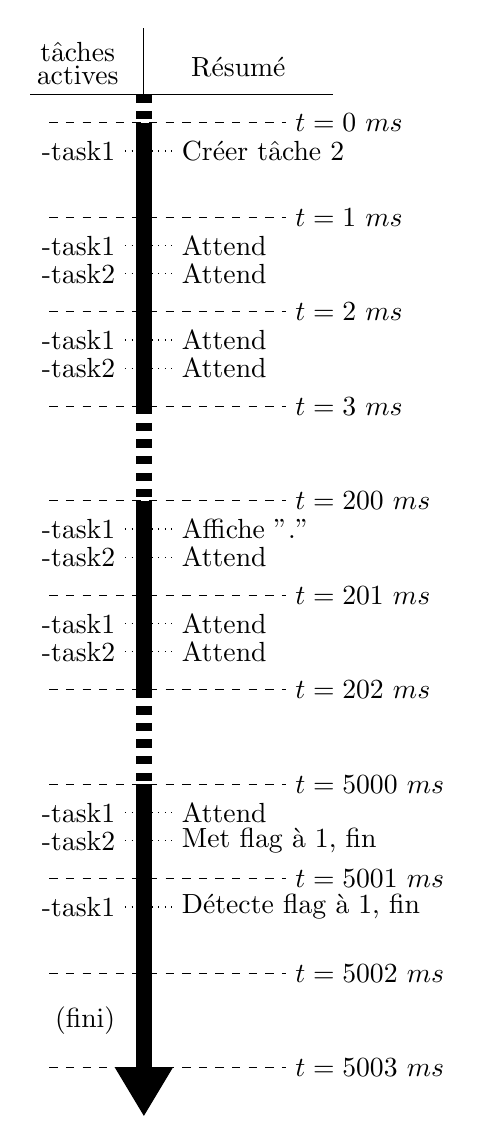
\begin{tikzpicture}[scale=1.2]

    % \draw [help lines] (-1, 0) grid (2, 12);

    \draw node at (-0.7, 11.75) {tâches};
    \draw node at (-0.7, 11.50) {actives};
    \draw node at ( 1, 11.595) {Résumé};

    % \draw [line width=0.5mm] (-1.2, 11.25) -- (2, 11.25);
    \draw (-1.2, 11.3) -- (2, 11.3);

    \draw  (0, 12) -- (0, 11.3);
    \draw [line width=2mm, dashed] (0, 11.3) -- (0, 11);
    \draw [line width=2mm        ] (0, 11) -- (0,  8);
    \draw [line width=2mm, dashed] (0,  8) -- (0,  7);
    \draw [line width=2mm        ] (0,  7) -- (0,  5);
    \draw [line width=2mm, dashed] (0,  5) -- (0,  4);
    \draw [line width=2mm        ] (0,  4) -- (0,  1);
    \draw [fill=black] (-0.3, 1) -- (0.3, 1) -- (0, 0.5) -- cycle;

    \draw [dashed] (-1, 11) -- (1.5, 11) node [right] {$t=   0 \ ms$};
    \draw [dashed] (-1, 10) -- (1.5, 10) node [right] {$t=   1 \ ms$};
    \draw [dashed] (-1,  9) -- (1.5,  9) node [right] {$t=   2 \ ms$};
    \draw [dashed] (-1,  8) -- (1.5,  8) node [right] {$t=   3 \ ms$};
    \draw [dashed] (-1,  7) -- (1.5,  7) node [right] {$t= 200 \ ms$};
    \draw [dashed] (-1,  6) -- (1.5,  6) node [right] {$t= 201 \ ms$};
    \draw [dashed] (-1,  5) -- (1.5,  5) node [right] {$t= 202 \ ms$};
    \draw [dashed] (-1,  4) -- (1.5,  4) node [right] {$t=5000 \ ms$};
    \draw [dashed] (-1,  3) -- (1.5,  3) node [right] {$t=5001 \ ms$};
    \draw [dashed] (-1,  2) -- (1.5,  2) node [right] {$t=5002 \ ms$};
    \draw [dashed] (-1,  1) -- (1.5,  1) node [right] {$t=5003 \ ms$};

    \draw [dotted] (-0.2, 10.7) node[left]{-task1} -- (0.3, 10.7) node[right]{Créer tâche 2};

    \draw [dotted] (-0.2,  9.7) node[left]{-task1} -- (0.3,  9.7) node[right]{Attend};
    \draw [dotted] (-0.2,  9.4) node[left]{-task2} -- (0.3,  9.4) node[right]{Attend};

    \draw [dotted] (-0.2,  8.7) node[left]{-task1} -- (0.3,  8.7) node[right]{Attend};
    \draw [dotted] (-0.2,  8.4) node[left]{-task2} -- (0.3,  8.4) node[right]{Attend};

    \draw [dotted] (-0.2,  6.7) node[left]{-task1} -- (0.3,  6.7) node[right]{Affiche "."};
    \draw [dotted] (-0.2,  6.4) node[left]{-task2} -- (0.3,  6.4) node[right]{Attend};

    \draw [dotted] (-0.2,  5.7) node[left]{-task1} -- (0.3,  5.7) node[right]{Attend};
    \draw [dotted] (-0.2,  5.4) node[left]{-task2} -- (0.3,  5.4) node[right]{Attend};

    \draw [dotted] (-0.2,  3.7) node[left]{-task1} -- (0.3,  3.7) node[right]{Attend};
    \draw [dotted] (-0.2,  3.4) node[left]{-task2} -- (0.3,  3.4) node[right]{Met flag à 1, fin};

    \draw [dotted] (-0.2,  2.7) node[left]{-task1} -- (0.3,  2.7) node[right]{Détecte flag à 1, fin};

    \draw          (-0.2,  1.5) node[left]{(fini)};


\end{tikzpicture}
\caption{Chronologie de l'exemple de programmation asynchrone}
\end{wrapfigure}

La figure ci-contre montre la chronologie de l'exemple. A noter que le temps
d'exécution est donné à titre indicatif et ne correspond pas à une échelle de temps réelle.

\vspace{0.5cm}

Le programme commence par créer et initialiser l'ordonanceur (ligne \ref{lst:ex_async:start-init-scheduler}
-\ref{lst:ex_async:end-init-scheduler}). C'est à dire que de la mémoire est alloué pour les tâches, que les
éléments du tableau \texttt{running} sont tous mis à \texttt{false} et que les autres variables de
l'ordonanceur sont également initialisées.
Ensuite, la tâche 1 est créée et ajoutée à l'ordonanceur. Cela est réalisé par l'appelle de la fonction
\texttt{add\_task}. Cette fonction cherche la première place libre dans la zone mémoire allouée à cet effet
dans le tas, initialise une nouvelle tâche à cet endroit et renvoie un pointeur vers cette dernière.
Le context de la tâche est ensuite initialisé par sa fonction relative (ici\newline \texttt{ASYNC\_task1\_init})
(lignes \ref{lst:ex_async:start-init-task1}-\ref{lst:ex_async:end-init-task1}).
Enfin, le programme entre dans une boucle et exécute la fonction \texttt{run\_scheduler} tant que
des tâches se trouvent active dans l'ordonanceur.

Au début de l'exécution, seule la tâche 1 se trouve active, elle est alors exécutée. Ligne
\ref{lst:ex_async:start-task1}, le contexte d'exécution de la tâche 1 est récupéré et l'état de la tâche
est vérifié. La plupart des tâches sont des machines à états finis \footnotemark. Dans le cas de la tâche
1, elle se trouve au début dans l'état \texttt{TASK1\_INIT}, elle affiche donc le message "Task 1 : Start",
créer la tâche 2 en l'ajoutant à l'ordonanceur, affiche "Task 1 : Wait" et passe à l'état \texttt{TASK1\_WAIT}.

La tâche 1 est alors mise en pause et la tâche 2 est exécutée. Cette dernière est une tâche simulant
une opération prenant du temps. Elle démarre tout d'abord un timer de 5000 ms et vérifie à chaque nouvelle
exécution si ce temps s'est écoulé. Lorsque c'est le cas, la tâche 2 se retire de l'ordonanceur. Quand la
tâche 1 détecte la fin d'exéctution de la tâche 2 (via la mise à jour du drapeau "\texttt{task2\_done}"), elle
affiche "Task 1 : End" et se retire également de l'ordonanceur. Dans le cas contraire, la tâche 1 continue
d'afficher des points toutes les 200 ms grâce à un timer propre. Ainsi, 25 points sont affichés correspondant
à un point toutes les 200 ms pendant 5 secondes. 

\end{minipage}

\footnotetext{Machine à état : Une machine à état (ou automate fini) est un modèle de calcul utilisé pour
représenter des systèmes avec un nombre fini d'états. Ce modèle est utilisé dans divers domaines comme les
protocoles de communication, les jeux vidéo, les systèmes embarqués, etc.}

